\documentclass{brounst}

\begin{document}

%====================================================================
% PARAMÈTRES LOCAUX AU DOCUMENT
%====================================================================
\titleformat{\section}
  {\normalfont\LARGE\bfseries}   % style du titre
  {\thesection}                  % numéro
  {1em}                          % espace entre numéro et titre
  {\MakeUppercase}                             % rien avant le titre
  [\titlerule]                   % --- ce qui vient APRÈS, collé au titre

\titlespacing*{\section}
  {0pt}                          % indentation gauche
  {3.5ex plus 1ex minus .2ex}    % espace AVANT le titre
  {2.0ex plus .2ex}              % espace APRÈS la ligne (avant le texte suivant)

% -- Listes (itemize) --------------------------------------------------
\renewcommand{\labelitemi}{$\bullet$}
\renewcommand{\labelitemii}{$\circ$}
\renewcommand{\labelitemiii}{$-$}
\renewcommand{\labelitemiv}{$\circ$}

% -- Titres ----------------------------------------------------------------
\titlespacing*{\subsubsection}{15pt}{\baselineskip}{0.2\baselineskip} % 1er élément indentation et 2ème espace en-dessous

% -- Divers ------------------------------------------------------------------
\tolerance=5000 %augementation de la tolérance des coupures


%====================================================================
% PAGE DE TITRE 
%====================================================================
\maketitleSimple

%====================================================================
% EN-TÊTE ET PIED DE PAGE (numérotation arabe)
%====================================================================
\pagenumbering{arabic}
% \fancystandard
\fancyOnlyFoot

%====================================================================
% CONTENU
%====================================================================
\section{Introduction}

Ce document sert à reproduire un modèle Latex défini et une méthodologie pour créer des rapports Latex.

\section{Installation sur Linux}

Il s'agit de la méthode que j'utilise pour faire du latex.

\vspace{1em}
Les logiciels à télécharger sont : 
\begin{itemize}
    \item \href{https://code.visualstudio.com/}{Visual studio code} comme éditeur de texte
    \item \href{https://miktex.org/download}{MikTex} pour pouvoir coder en Latex
    \item \href{https://strawberryperl.com/}{Strawberry Perl} pour pouvoir utiliser VScode et Latex
\end{itemize}

Il faut installer l'extension LaTex Workshop dans VScode.
\begin{figure}[H]


\includegraphics[width=7cm]{latex_workshop.jpg}
\end{figure}

Il faut aussi ouvrir MikTex Console et contrôler que tous les packages sont à jour.
\begin{figure}[H]


\includegraphics[width=14cm]{miktex_update.jpg}
\end{figure}

Il est alors possible de créer un rapport latex en reprenant ce modèle.

\break
\section{Exemple de code Latex}

\subsection{Font}
\subsubsection{Size}
\begin{itemize}
  \item {\tiny tiny}
  \item {\scriptsize scriptsize}
  \item {\footnotesize footnotesize}
  \item {\small small}
  \item {\normalsize normalsize}
  \item {\large large}
  \item {\LARGE LARGE}
  \item {\huge huge}
  \item {\Huge Huge}
\end{itemize}
\subsubsection{Decoration}
\underline{Sous-ligné} : \verb|\underline{}|

\textbf{gras} : \verb|\textbf{}|

\textit{italic} : \verb|\textit{}|



\subsection{Lien -- marque page}\label{sec:lien}
\subsubsection{note en pied de page}
A bove ante, ab asino retro, a stulto undique caveto\footnote{Prends garde au bœuf par devant, à l'âne par derrière, à l'imbécile par tous les côtés.} \verb|\footnote{}|

\subsubsection{Figure référence}

Voir Figure \ref{sec:lien} à la page \pageref{sec:lien}  \verb|\label{} \ref{}  \pageref{}|

\subsubsection{Url}
\url{https://fr.wikipedia.org/wiki/Liste_de_locutions_latines}  \verb|\url{}|

\href{https://fr.wikipedia.org/wiki/Liste_de_locutions_latines}{Locutions latines} \verb|\href{}{}|

\subsubsection{Source biblio}

\textcit{Oh punaise}\cite{agressin} \verb|\cite{} #référence biblio auto|

\textcit{Oh punaise}\citemanuel{Gressin} \verb|\citemanuel{} #référence manuel|

% === FIGURE =================================================================================
\subsection{Figure}

\begin{verbatim}
\begin{figure}[H]
    \centering
		\includegraphics[width=2cm]{HEIG-VD_logotype-baseline_rouge-rvb.png}
    \caption[Logo heig]{Logo heig \footnotemark}
    \label{fig:latex}
\end{figure}
\footnotetext{source : \url{https://heig-vd.ch/}}
\end{verbatim}
\begin{figure}[H]
    \centering
		
\includegraphics[width=2cm]{heig_hes.jpg}
    \caption[Logo heig]{Logo heig \footnotemark}
    \label{fig:latex}
\end{figure}
\footnotetext{source : \url{https://heig-vd.ch/}}


% === TABLEAU =================================================================================
\subsection{Tableau}



\begin{verbatim}
\begin{table}[H]
  \centering
  \renewcommand{\arraystretch}{1.3}
  \begin{tabularx}{\textwidth}{>{\centering\bfseries}C{1.5cm} X X}
    \toprule
    \rowcolor{tableheader}
    \textbf{Groupe} & \textbf{Appareil photo} & \textbf{Trépied} \\
    \midrule
    1 & Canon EOS 5D Mark III avec obj.\ de 20\,mm & Rodeon piXpert \\
    \rowcolor{codebg}
      ...
    4 & Canon EOS 700D avec obj.\ de 10\,mm & Trépied avec Rollei 200 Mark II \\
    \bottomrule
  \end{tabularx}
  \caption{Répartition du matériel par groupe}
\end{table}
\end{verbatim}
\begin{table}[H]
  \centering
  \renewcommand{\arraystretch}{1.3}
  \begin{tabularx}{\textwidth}{>{\centering\bfseries}C{1.5cm} X Y}
    \toprule
    \rowcolor{tableheader}
    \textbf{Groupe} & \textbf{Appareil photo} & \textbf{Trépied} \\
    \midrule
    1 & Canon EOS 5D Mark III avec obj.\ de 20\,mm & Rodeon piXpert \\
    \rowcolor{codebg}
    2 & QooCam 8K & Trépied standard \\
    3 & Canon EOS 5D Mark III avec obj.\ de 14\,mm & Trépied avec Rollei 200 Mark II \\
    \rowcolor{codebg}
    4 & Canon EOS 700D avec obj.\ de 10\,mm & Trépied avec Rollei 200 Mark II \\
    \bottomrule
  \end{tabularx}
  \caption{Tableau sur la largeur autorisée}
\end{table}
\begin{verbatim}
\begin{table}[H]
  \centering
  \renewcommand{\arraystretch}{1.3}
  \begin{tabular}{>{\bfseries}L{1.5cm} C{3.5cm}  C{3.5cm} }
    \toprule
    \rowcolor{tableheader}
    \textbf{Groupe} & \textbf{Appareil photo} & \textbf{Trépied} \\
    \midrule
    1 & Canon EOS 5D Mark III avec obj.\ de 20\,mm & Rodeon piXpert \\
    \rowcolor{codebg}
      ...
    4 & Canon EOS 700D avec obj.\ de 10\,mm & Trépied avec Rollei 200 Mark II \\
    \bottomrule
  \end{tabular}
  \caption{Répartition du matériel par groupe}
\end{table}
\end{verbatim}
\begin{table}[H]
  \centering
  \renewcommand{\arraystretch}{1.3}
  \begin{tabular}{>{\bfseries}L{1.5cm} C{3.5cm}  C{3.5cm} }
    \toprule
    \rowcolor{tableheader}
    \textbf{Groupe} & \textbf{Appareil photo} & \textbf{Trépied} \\
    \midrule
    1 & Canon EOS 5D Mark III avec obj.\ de 20\,mm & Rodeon piXpert \\
    \rowcolor{codebg}
    2 & QooCam 8K & Trépied standard \\
    3 & Canon EOS 5D Mark III avec obj.\ de 14\,mm & Trépied avec Rollei 200 Mark II \\
    \rowcolor{codebg}
    4 & Canon EOS 700D avec obj.\ de 10\,mm & Trépied avec Rollei 200 Mark II \\
    \bottomrule
  \end{tabular}
  \caption{Tableau avec largeur fixée}
\end{table}


\begin{verbatim}
 \renewcommand{\arraystretch}{1.3}
\begin{longtable}{lC{2.3cm}C{2.5cm}C{3.2cm}C{1.8cm}}
   ...
\end{longtable}
\end{verbatim}
{
 \renewcommand{\arraystretch}{1.3}
\begin{longtable}{lC{2.3cm}C{2.5cm}C{3.2cm}C{1.8cm}}
 

  % En-tête première page
  \toprule
  \rowcolor{tableheader}
  \textbf{Focale [mm]} & \textbf{Tile count (H)} & \textbf{Stopover count (V)} & \textbf{Angles U/L (V)} & \textbf{Total} \\
  \midrule
  \endfirsthead

  % En-tête pages suivantes
  \toprule
  \rowcolor{tableheader}
  \textbf{Focale [mm]} & \textbf{Tile count (H)} & \textbf{Stopover count (V)} & \textbf{Angles U/L (V)} & \textbf{Total} \\
  \midrule
  \endhead

  % Pied de page (sauf dernière)
  \midrule
  \multicolumn{5}{r}{\emph{Suite page suivante}} \\
  \endfoot

  % Pied de page dernière page
  
  \endlastfoot

  % Données
  10 \emph{(portrait)}  & 5   & 2  & 45° / $-$45°   & 10  \\
  \rowcolor{codebg}
  14 \emph{(portrait)}  & 6--7 & 3  & 60° / $-$60°   & 18  \\
  20 \emph{(portrait)}  & 8   & 3  & 60° / $-$60°   & 24  \\
  \rowcolor{codebg}
  24 \emph{(portrait)}  & 9   & 4  & 68° / $-$68°   & 36  \\
  28 \emph{(portrait)}  & 11  & 4  & 68° / $-$68°   & 44  \\
  \rowcolor{codebg}
  \bottomrule
  \caption{Tableau sur plusieurs page}
  \label{tab:recouvrodeon} 
\end{longtable}
}


\begin{table}[H]
    \centering
{\tiny
        \renewcommand{\arraystretch}{2.5}
        \fontsize{10pt}{10pt}\selectfont
        \begin{tabular}{|>{\footnotesize}L{1.5cm}|>{\footnotesize}L{3cm}|>{\footnotesize}L{3cm}|}
            \hline
            \rowcolor{gray!30} % Couleur de fond de l'en-tête
            \textbf{Paires d'images} & \vphantom{g}\textbf{IA LightGlue} & \vphantom{g}\textbf{Algorithme de type SIFT de Agisoft}\\
            \hline
        \end{tabular}
        \renewcommand{\arraystretch}{1.5}
        \begin{tabular}{|>{\footnotesize}L{1.5cm}|>{\footnotesize}L{3cm}|>{\footnotesize}L{3cm}|}
            1 &Valide : 134 points \newline \underline{Invalide : 29 points}\newline \vspace{0.5em} Total : 163 points  &  Valide : 5 points \newline \underline{Invalide : 5 points}\newline  \vspace{0.5em} Total : 10 points \\
            \hline
            2 & Valide : 19 points \newline \underline{Invalide : 28 points}\newline \vspace{0.5em}  Total : 47 points & Valide : 0 points \newline \underline{Invalide : 0 points} \newline \vspace{0.5em}  Total : 0 points \\
            \hline
        \end{tabular}}
        \caption{Tableau standard}
        \label{tab:comp}
\end{table}



% === BOXES =================================================================================
\subsection{Boxes}

\begin{verbatim}
\reponseplace{}
\end{verbatim}
\reponseplace{}

\begin{verbatim}
\reponseplaceautoheight{}
\end{verbatim}
\reponseplaceautoheight{Alea jacta est}

\begin{verbatim}
\begin{warningbox}
  ...
\end{warningbox}
\end{verbatim}
\begin{warningbox}
  Cogito, ergo sum 
\end{warningbox}

\begin{verbatim}
\begin{infobox}
  ...
\end{infobox}
\end{verbatim}
\begin{infobox}[Linux]
  Errare humanum est
\end{infobox}


\begin{verbatim}
\aretenir{}
\definition{}
\end{verbatim}
\aretenir{Element important}
\definition{Définition d'un mot}
% === Code =================================================================================
\subsection{Impression de code}
\begin{verbatim}
\begin{lstlisting}[style=standard]
  ...
\end{lstlisting}
\end{verbatim}
\begin{lstlisting}[style=standard]
brutes/
|---- pano1/
|     |---- 7W4C7165.JPG
|     |---- 7W4C7166.JPG
|     `---- ...
|---- pano2/
|     |---- 7W4C7191.JPG
|     |---- 7W4C7192.JPG
|     `---- ...
|---- pano3/ ...
|---- pano4/ ...
`---- pano5/ ...
\end{lstlisting}

\begin{verbatim}
\begin{lstlisting}[style=sqlstyle]
  ...
\end{lstlisting}
\end{verbatim}
\begin{lstlisting}[style=sqlstyle]
SELECT 
  *
FROM test_table tt 
INNER JOIN lien_table lt on tt.id=lt.id
WHERE tt.nom='Bruno'
\end{lstlisting}
\begin{verbatim}
\begin{lstlisting}[style=python]
  ...
\end{lstlisting}
\end{verbatim}
\begin{lstlisting}[style=python]
a = 5
for i in range(5):
  print(a)
\end{lstlisting}

% === LISTES =================================================================================
\subsection{Listes}

\begin{verbatim}
  \begin{itemize}
    ...
  \end{itemize}
\end{verbatim}
\begin{itemize}
  \item Absentem lædit, qui cum ebrio litigat
  \begin{itemize}
      \item \href{https://code.visualstudio.com/}{Visual studio code} comme éditeur de texte
    \end{itemize}
  \item Orientation externe
  \begin{itemize}
      \item La position de l'image cible $S_{cible}=[X_{cible},Y_{cible},Z_{cible}]$
      \item L'orientation de l'image $R_\omega, R_\phi, R_\kappa$
  \end{itemize}
  \item Calibration interne (modèle \og Frame \fg de Agisoft)
  \begin{itemize}
      \item Le point principal d'autocollimation $PPA=[x_c,y_c]$
  \end{itemize}
  \item un facteur de proximité spatiale, défini par la formule : \\
        $
    \text{poids}_{\text{distance}} = 
    \begin{cases}
    1 - \dfrac{\text{dist}}{70}, & \text{si } \text{dist} < 70 \\
    0.0000001, & \text{sinon}
    \end{cases}
    $\\ \\
    \textit{\small La valeur déterminante de 70m a été choisie de manière empirique.}\\
\item un facteur d’orientation, calculé à l’aide du produit scalaire entre les vecteurs d’orientation (résultant en une valeur entre -1 et 1, soit le cosinus de l’angle).
\end{itemize}

\begin{verbatim}
  \begin{enumerate}
    ...
  \end{enumerate}
\end{verbatim}
\begin{enumerate}
  \raggedright % pas de justification
  \item Amare et sapere vix deo conceditur
  \begin{enumerate}
      \item Amicus certus in re incerta cernitur
    \end{enumerate} 
  \item An nescis, mi fili, quantilla prudentia mundus regatur
\end{enumerate}




% === MATH =================================================================================
\subsection{Fonction mathématique}

\subsubsection{Boxed}
\begin{equation}
    \boxed{m = F - \frac{k^TFR(M-S)}{k^T R(M-S)}}\\
    \label{colin}
\end{equation}
\subsubsection{Alignement}
\begin{align*}
    x_m&=x_c+f\cdot\frac{r_{11}(X_M-X_S)+r_{21}(Y_M-Y_S)+r_{31}(Z_M-Z_S)}{r_{13}(X_M-X_S)+r_{23}(Y_M-Y_S)+r_{33}(Z_M-Z_S)}\\
    y_m&=y_c+f\cdot\frac{r_{12}(X_M-X_S)+r_{22}(Y_M-Y_S)+r_{32}(Z_M-Z_S)}{r_{13}(X_M-X_S)+r_{23}(Y_M-Y_S)+r_{33}(Z_M-Z_S)}\\
    z_m&=0
\end{align*}
\subsubsection{Description}
\begin{align*}
    \descrVarEq{\scu^{cam}=(o,x,y,z)}{Système de coordonnée de la caméra}\\
    \descrVarEq{x,y}{Centre du capteur de l'image}\\
    \descrVarEq{z}{Axe de la visée de l'appareil photo}\\
    \descrVarEq{\scu^{glob}=(O,X,Y,Z)}{Système de coordonnées globale}\\
    \descrVarEq{m=[x_m,y_m,0]}{Coordonnée d'un point terrain sur le capteur, z=0 dans $\scu^{cam}$}\\
    \descrVarEq{M=[X_M,Y_M,Z_M]}{Coordonnée d'un point terrain dans $\scu^{glob}$}\\
    \descrVarEq{S=[X_S,Y_S,Z_S]}{Coordonnée du point de la caméra dans $\scu^{glob}$}\\
    R_{glob}^{cam}=R_\omega\cdot R_\phi\cdot R_\kappa=\begin{bmatrix}
    r_{11}&r_{21}&r_{31}\\
    r_{12}&r_{22}&r_{32}\\
    r_{13}&r_{23}&r_{33}
    \end{bmatrix}\textrm{ : }&\textrm{Matrice de rotation du $\scu^{glob}$vers $\scu^{cam}$}\\
    \descrVarEq{F=[x_c,y_c,-f]}{Point S dans $\scu^{cam}$}\\
    &\textrm{(Distance focale $f$)}\\
    &\textrm{($x_c,y_c$ sont égales à 0 dans un modèle théorique)}\\
\end{align*}
\subsubsection{Suppression - va vers 0}
$$ \Delta h = \frac{d'_{AB} \cdot \cos(\zeta_A) - d'_{BA} \cdot \cos(\zeta_B)}{2} + (1-k) \frac{\cancelto{0}{(d'_{AB} \cdot\sin \zeta_A)^2 - (d'_{BA} \cdot\sin \zeta_B)^2}}{4r} + \frac{(I_A - S_B) - (I_B - S_A)}{2} $$

\subsubsection{Divers}
\begin{equation}
    \label{eq:transdlt}
    L=\frac{-1}{\sqrt{L^2_9+L^2_{10}+L^2_{11}}}
\end{equation} 
\begin{align*}
    x_c&\approx L^2(L_1L_9+L_2L_{10}+L_3L_{11})\\
    y_c&\approx L^2(L_5L_9+L_6L_{10}+L_7L_{11})\\
    c_x&\approx\sqrt{L^2(L^2_1+L^2_2+L^2_3)-x^2_c}\\
    c_y&\approx\sqrt{L^2(L^2_5+L^2_6+L^2_7)-y^2_c}\\
    p&\approx  (c_x+c_y)/2
\end{align*}
$$r_{11}\approx\frac{L(x_cL_9-L_1)}{c_x},r_{12}\approx\frac{L(y_cL_9-L_5)}{c_y},r_{13}\approx L\cdot L_9 $$
$$r_{21}\approx\frac{L(x_cL_{10}-L_2)}{c_x},r_{22}\approx\frac{L(y_cL_{10}-L_6)}{c_y},r_{23}\approx L\cdot L_{10} $$
$$r_{31}\approx\frac{L(x_cL_{11}-L_3)}{c_x},r_{32}\approx\frac{L(y_cL_{11}-L_7)}{c_y},r_{33}\approx L\cdot L_{11} $$
\begin{equation*}
    \begin{bmatrix}
        X_S\\Y_S\\Z_S
    \end{bmatrix}\approx -
    \begin{bmatrix}
        L_1&L_2&L_3\\
        L_5&L_6&L_7\\
        L_9&L_{10}&L_{11}\\
    \end{bmatrix}^{-1}\cdot 
    \begin{bmatrix}
        L_4\\L_8\\1
    \end{bmatrix}
\end{equation*}

\subsection{Style de texte}

\verb|\textcit{...}|

\textcit{Fleur en bouquet fanne, mais jamais ne renait}

\verb|\reminterne{...}|

\reminterne{Remarques internes, élément à modifier}

\verb|\remintbox{...}|

\remintbox{Remarque internes, élément à modifier}

\verb|\bfit{...}|

\bfit{Italic gras}

\verb|\paragraphtitle{...}|

\paragraphtitle{Titre de paragaphe}

\subsection{Figures dessinées internes}

\begin{figure}[H]
    \centering
    \begin{tikzpicture}[
        node distance=1cm,
        input/.style={circle, draw=link, thick, fill=link!8, minimum size=0.8cm},
        sum/.style={circle, draw=accent, thick, fill=accent!10, minimum size=1cm},
        actout/.style={circle, draw=accent, thick, fill=accent!20, minimum size=0.9cm}
    ]
        \node[input] (x0) at (0,2.0) {$x_0{=}1$};
        \node[input] (x1) at (0,0.9) {$x_1$};
        \node[input] (x2) at (0,0) {$x_2$};
        \node[input] (x3) at (0,-1.2) {$x_n$};
        \node at (0,-0.5) {$\vdots$};
        \node[sum] (sum) at (2.5,0.45) {$\sum$};
        \node[actout] (act) at (4.5,0.45) {$f$};
        \node[right=0.4cm of act] (y) {$\hat y$};
        \draw[-Latex] (x0) -- node[above,sloped,font=\scriptsize]{$w_0$} (sum);
        \draw[-Latex] (x1) -- node[above,sloped,font=\scriptsize]{$w_1$} (sum);
        \draw[-Latex] (x2) -- node[above,sloped,font=\scriptsize]{$w_2$} (sum);
        \draw[-Latex] (x3) -- node[below,sloped,font=\scriptsize]{$w_n$} (sum);
        \draw[-Latex] (sum) -- (act);
        \draw[-Latex] (act) -- (y);
    \end{tikzpicture}
    \caption{Exemple de graphique dessiné}
    \label{fig:perceptron}
\end{figure}
\begin{figure}[H]
    \centering
    \begin{tikzpicture}[
        node distance=0.6cm,
        neuron/.style={circle, draw=link, thick, fill=link!8, minimum size=0.7cm},
        neuronh/.style={circle, draw=accent, thick, fill=accent!10, minimum size=0.7cm},
        neurono/.style={circle, draw=accent, thick, fill=accent!20, minimum size=0.7cm}
    ]
        \foreach \i/\y in {1/1.2, 2/0.4, 3/-0.4, 4/-1.2}
            \node[neuron] (i\i) at (0,\y) {};
        \foreach \i/\y in {1/1.6, 2/0.8, 3/0, 4/-0.8, 5/-1.6}
            \node[neuronh] (h1\i) at (2.2,\y) {};
        \foreach \i/\y in {1/1.2, 2/0.4, 3/-0.4, 4/-1.2}
            \node[neuronh] (h2\i) at (4.4,\y) {};
        \foreach \i/\y in {1/0.4, 2/-0.4}
            \node[neurono] (o\i) at (6.6,\y) {};
        \foreach \i in {1,2,3,4}
            \foreach \j in {1,2,3,4,5}
                \draw[-Latex, gray!60] (i\i) -- (h1\j);
        \foreach \i in {1,2,3,4,5}
            \foreach \j in {1,2,3,4}
                \draw[-Latex, gray!60] (h1\i) -- (h2\j);
        \foreach \i in {1,2,3,4}
            \foreach \j in {1,2}
                \draw[-Latex, gray!60] (h2\i) -- (o\j);
        \node[align=center] at (0.0,-2.3) {\small Entrée};
        \node[align=center] at (2.2,-2.3) {\small Couche\\cachée 1};
        \node[align=center] at (4.4,-2.3) {\small Couche\\cachée 2};
        \node[align=center] at (6.6,-2.3) {\small Sortie};
    \end{tikzpicture}
    \caption{Exemple de graphique dessiné 2}
    \label{fig:mlp}
\end{figure}

\begin{figure}[H]
    \centering
    \begin{tikzpicture}[scale=0.62]
        \foreach \x in {0,...,4} {
            \foreach \y in {0,...,4} {
                \draw[gray!45] (\x,\y) rectangle ++(1,1);
            }
        }
        \draw[accent, very thick] (1,1) rectangle ++(3,3);
        \node[font=\scriptsize] at (2.5,4.6) {image d'entrée};

        \draw[-{Latex[length=3mm]}, thick, accent] (5.3,2.5) -- (7.3,2.5);
        \node[font=\scriptsize, align=center] at (6.3,3.1) {noyau $K$\\($3\times3$)};

        \foreach \x in {0,...,2} {
            \foreach \y in {0,...,2} {
                \draw[gray!45] (8+\x,1+\y) rectangle ++(1,1);
            }
        }
        \draw[accent, very thick, fill=accent!25] (9,2) rectangle ++(1,1);
        \node[font=\scriptsize] at (9.5,4.6) {image de sortie};
    \end{tikzpicture}
    \caption{Exemple de graphique dessiné 3}
    \label{fig:convolution-principe}
\end{figure}


\begin{figure}[H]
    \centering
    \begin{tikzpicture}[scale=0.55]
        \foreach \x in {0,...,4} {
            \foreach \y in {0,...,4} {
                \draw[link, thick] (\x,\y) rectangle ++(1,1);
            }
        }
        \draw[accent, ultra thick] (1,1) rectangle ++(3,3);
        \node[below] at (2.5,-0.5) {\small Image : grille régulière, voisinage fixe};
    \end{tikzpicture}
    \hspace{1.2cm}
    \begin{tikzpicture}[scale=0.55]
        \foreach \p in {(0.3,0.5), (1.2,2.8), (2.6,0.9), (3.8,3.4), (0.9,4.1), (4.2,1.6), (2.1,3.7), (3.3,0.4), (1.6,1.4), (4.6,4.2), (0.5,3.2), (2.9,2.2), (3.9,4.8), (1.0,0.2), (4.4,3.0)} {
            \fill[link] \p circle (2.5pt);
        }
        \fill[accent] (2.1,3.7) circle (3pt);
        \draw[accent, thick, dashed] (2.1,3.7) circle (1.1);
        \node[below] at (2.5,-0.5) {\small Nuage de points : ensemble non structuré};
    \end{tikzpicture}
    \caption{Exemple de graphique dessiné 4}
    \label{fig:image-vs-nuage}
\end{figure}
\begin{figure}[H]
    \centering
    \begin{tikzpicture}
        \begin{axis}[
            width=9cm, height=6cm,
            xlabel={$x$}, ylabel={$f(x)$},
            xmin=-6, xmax=6, ymin=-1.2, ymax=1.2,
            axis lines=middle,
            grid=major, grid style={gray!15},
            legend pos=south east,
            legend style={font=\small, draw=gray!40},
            samples=100, domain=-6:6,
            every axis plot/.append style={very thick},
        ]
            \addplot[link] {1/(1+exp(-x))};
            \addplot[accent] {tanh(x)};
            \legend{$\sigma(x)$, $\tanh(x)$}
        \end{axis}
    \end{tikzpicture}
    \caption{Exemple de graphique de fonction}
    \label{fig:plot-sigmoid-tanh}
\end{figure}

\begin{figure}[H]
    \centering
    \begin{tikzpicture}
        \begin{axis}[
            width=8.5cm, height=5.5cm,
            ybar, bar width=28pt,
            symbolic x coords={Classe A, Classe B, Classe C},
            xtick=data,
            ymin=0, ymax=0.85,
            ylabel={Probabilité $\mathrm{softmax}(z)_k$},
            nodes near coords,
            enlarge x limits=0.3,
            axis lines*=left,
            ymajorgrids, grid style={gray!15},
        ]
            \addplot[fill=accent!70, draw=accent] coordinates {(Classe A,0.659) (Classe B,0.242) (Classe C,0.099)};
        \end{axis}
    \end{tikzpicture}
    \caption{Exemple de graphique à barre}
    \label{fig:plot-softmax}
\end{figure}


\begin{figure}[H]
    \centering
    \begin{tikzpicture}[
        block/.style={rectangle, draw=link, thick, fill=link!8, minimum width=1.7cm, minimum height=1cm, align=center, font=\small},
        sum/.style={circle, draw=accent, thick, fill=accent!10, minimum size=0.7cm},
        node distance=1cm
    ]
        \node (zin) {$\mathbf{z}_{l-1}$};
        \node[block, right=0.9cm of zin] (ln1) {LN};
        \node[block, right=0.9cm of ln1] (msa) {MSA};
        \node[sum, right=0.7cm of msa] (add1) {$+$};
        \node[block, right=0.9cm of add1] (ln2) {LN};
        \node[block, right=0.9cm of ln2] (mlp) {MLP};
        \node[sum, right=0.7cm of mlp] (add2) {$+$};
        \node[right=0.6cm of add2] (zout) {$\mathbf{z}_l$};
        \draw[-Latex, thick] (zin) -- (ln1);
        \draw[-Latex, thick] (ln1) -- (msa);
        \draw[-Latex, thick] (msa) -- (add1);
        \draw[-Latex, thick] (add1) -- (ln2);
        \draw[-Latex, thick] (ln2) -- (mlp);
        \draw[-Latex, thick] (mlp) -- (add2);
        \draw[-Latex, thick] (add2) -- (zout);
        \draw[-Latex, thick] (zin) to[bend left=45] (add1);
        \draw[-Latex, thick] (add1) to[bend left=45] (add2);
    \end{tikzpicture}
    \caption{Exemple de diagramme}
    \label{fig:vit-block}
\end{figure}

\begin{figure}[H]
    \centering
    \begin{tikzpicture}[
        stepbox/.style={rectangle, rounded corners, draw=accent, thick, fill=accent!8, minimum width=3.5cm, minimum height=1.1cm, align=center, font=\small},
        arr/.style={-{Latex[length=2.5mm]}, thick, accent},
        dashedarr/.style={-{Latex[length=2.5mm]}, thick, accent, dashed}
    ]
        \node[stepbox] (comp) {1. Compréhension\\du problème};
        \node[stepbox, right=0.6cm of comp] (acq) {2. Acquisition};
        \node[stepbox, right=0.6cm of acq] (prep) {3. Préparation};
        \node[stepbox, below=0.9cm of prep] (mod) {4. Modélisation};
        \node[stepbox, left=0.6cm of mod] (eval) {5. Évaluation};
        \node[stepbox, left=0.6cm of eval] (comm) {6. Communication\\\& déploiement};
        \draw[arr] (comp) -- (acq);
        \draw[arr] (acq) -- (prep);
        \draw[arr] (prep) -- (mod);
        \draw[arr] (mod) -- (eval);
        \draw[arr] (eval) -- (comm);
        \draw[dashedarr] (comm.north) -- (comp.south);
    \end{tikzpicture}
    \caption{Exemple de diagramme 1}
    \label{fig:workflow-ds}
\end{figure}

\begin{figure}[H]
    \centering
    \begin{tikzpicture}[
        stepbox/.style={rectangle, rounded corners, draw=link, thick, fill=link!8, minimum width=2.6cm, minimum height=1cm, align=center, font=\small},
        arr/.style={-{Latex[length=2.5mm]}, thick, link}
    ]
        \node[stepbox] (img) {Image\\Sentinel-2};
        \node[stepbox, right=0.5cm of img] (attr) {Calcul\\d'attributs};
        \node[stepbox, right=0.5cm of attr] (train) {Entraînement\\Random Forest};
        \node[stepbox, right=0.5cm of train] (pred) {Carte\\d'occupation du sol};
        \draw[arr] (img) -- (attr);
        \draw[arr] (attr) -- (train);
        \draw[arr] (train) -- (pred);
    \end{tikzpicture}
    \caption{Exemple de diagramme très simple}
    \label{fig:chaine-teledetection}
\end{figure}


\subsection{Figures 3D dessinées internes}

\subsubsection{Système de coordonnées 3D}

\begin{figure}[H]
    \centering
    \begin{tikzpicture}
        \begin{axis}[
            width=7cm, height=7cm,
            view={115}{20},
            axis lines=center,
            xlabel={$X$}, ylabel={$Y$}, zlabel={$Z$},
            xmin=-0.5, xmax=2.8, ymin=-0.5, ymax=2.8, zmin=-0.5, zmax=2.8,
            ticks=none,
        ]
            \addplot3[-{Latex[length=3mm]}, ultra thick, link] coordinates {(0,0,0) (2.3,0,0)};
            \addplot3[-{Latex[length=3mm]}, ultra thick, accent] coordinates {(0,0,0) (0,2.3,0)};
            \addplot3[-{Latex[length=3mm]}, ultra thick, myreddark] coordinates {(0,0,0) (0,0,2.3)};
        \end{axis}
    \end{tikzpicture}
    \caption{Système de coordonnées 3D (repère orthonormé $X,Y,Z$)}
    \label{fig:repere3d}
\end{figure}

\begin{tikzpicture}
  \draw [->] (0,0) -- (1,0,0) node [right] {$x$};
  \draw [->] (0,0) -- (0,1,0) node [above] {$y$};
  \draw [->] (0,0) -- (0,0,1) node [below left] {$z$};

  \pgfpathcircle{\pgfpointcylindrical{80}{1}{.5}}{2pt}
  \pgfusepath{fill}

  \draw[red] (0,0) -- (0,0,.5) -- +(80:1);
\end{tikzpicture}

\begin{tikzpicture}[->]
  \draw (0,0,0) -- (xyz spherical cs:radius=1);
  \draw (0,0,0) -- (xyz spherical cs:radius=1,latitude=90);
  \draw (0,0,0) -- (xyz spherical cs:radius=1,longitude=90);
\end{tikzpicture}

\subsubsection{Cube}

\begin{figure}[H]
    \centering
    % Cube dessiné en TikZ pur (sans pgfplots) : on définit les axes x, y, z comme des
    % vecteurs 2D (projection cavalière) puis on ne trace que les 3 faces visibles,
    % avec un dégradé d'une même teinte pour simuler un éclairage venant du haut.
    \begin{tikzpicture}[
        x={(-0.87cm,-0.5cm)}, y={(0.87cm,-0.5cm)}, z={(0cm,1cm)},
        scale=2.2, line join=round, line cap=round,
    ]
        % Les 3 faces tracées se rejoignent toutes au sommet le plus proche du lecteur (1,1,1) ;
        % les 3 autres faces (touchant le sommet opposé (0,0,0)) restent cachées derrière.
        \draw[fill=link!25, draw=black, thick] (1,0,0) -- (1,1,0) -- (1,1,1) -- (1,0,1) -- cycle; % face gauche
        \draw[fill=link!45, draw=black, thick] (0,1,0) -- (1,1,0) -- (1,1,1) -- (0,1,1) -- cycle; % face droite
        \draw[fill=link!70, draw=black, thick] (0,0,1) -- (1,0,1) -- (1,1,1) -- (0,1,1) -- cycle; % face du haut
    \end{tikzpicture}
    \caption{Cube en 3D avec faces visibles}
    \label{fig:cube3d}
\end{figure}

\subsubsection{Sphère}

\begin{figure}[H]
    \centering
    \begin{tikzpicture}
        \begin{axis}[
            width=7cm, height=7cm,
            view={115}{20},
            axis lines=none,
            z buffer=sort,
            hide axis,
        ]
            \addplot3[
                surf, shader=faceted, draw=link, fill=link!25, opacity=0.9,
                domain=0:360, domain y=-90:90,
                samples=18, samples y=10,
            ] ({cos(x)*cos(y)}, {sin(x)*cos(y)}, {sin(y)});
        \end{axis}
    \end{tikzpicture}
    \caption{Sphère générée par une surface paramétrique}
    \label{fig:sphere3d}
\end{figure}

\subsubsection{Graphiques de fonctions 3D}

\begin{figure}[H]
    \centering
    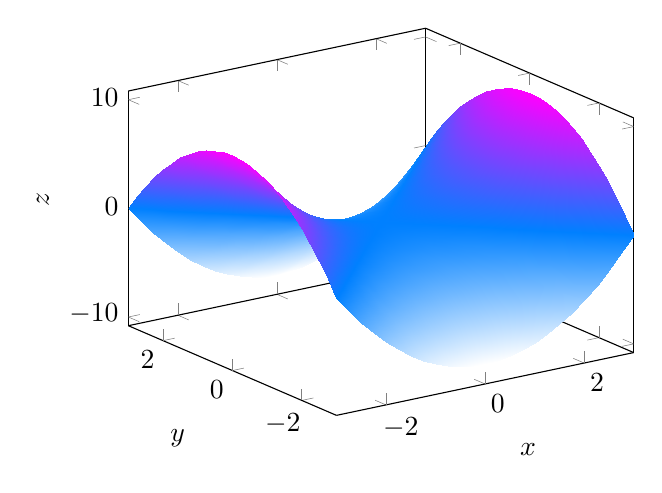
\begin{tikzpicture}
        \begin{axis}[
            width=8cm, height=6.5cm,
            view={-35}{25},
            xlabel={$x$}, ylabel={$y$}, zlabel={$z$},
            colormap/cool,
        ]
            \addplot3[
                surf, shader=interp,
                domain=-3:3, domain y=-3:3, samples=25,
            ] {x^2 - y^2};
        \end{axis}
    \end{tikzpicture}
    \caption{Paraboloïde hyperbolique $z=x^2-y^2$}
    \label{fig:fonction3d-selle}
\end{figure}

\begin{figure}[H]
    \centering
    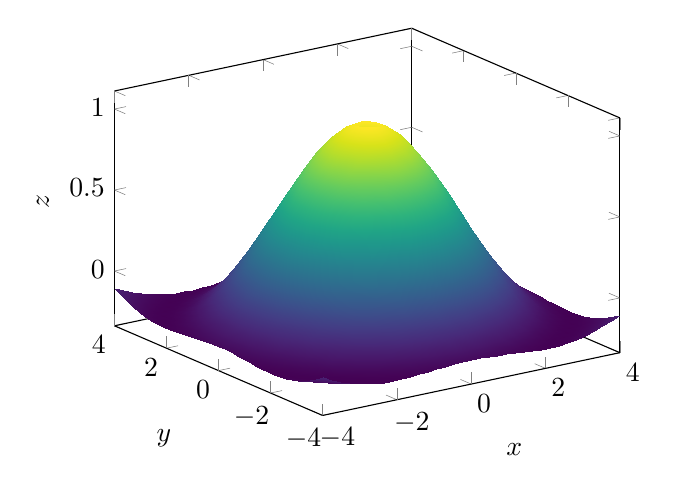
\begin{tikzpicture}
        \begin{axis}[
            width=8cm, height=6.5cm,
            view={-35}{25},
            xlabel={$x$}, ylabel={$y$}, zlabel={$z$},
            colormap/viridis,
        ]
            \addplot3[
                surf, shader=interp,
                domain=-4:4, domain y=-4:4, samples=35,
            ] {sin(deg(sqrt(x^2+y^2)+0.0001))/(sqrt(x^2+y^2)+0.0001)};
        \end{axis}
    \end{tikzpicture}
    \caption{Fonction \og sombrero \fg{} $z=\sin(r)/r$}
    \label{fig:fonction3d-sombrero}
\end{figure}

\newpage

%====================================================================
% BIBLIOGRAPHIE
%====================================================================
\bibliographystyle{apalike-fr}
\renewcommand{\refname}{Bibliographie} %Pour les articles
\renewcommand{\bibname}{Bibliographie} %Pour les thèses/livres
\bibliography{biblio}
\nocite{*}


\end{document}
